% === Table 1: Main Results ===

% === Fig 3: Evolution Trajectory (D3 version) ===
% Fig 3: Evolution Trajectory (D3 version)
\begin{figure*}[t]
\centering
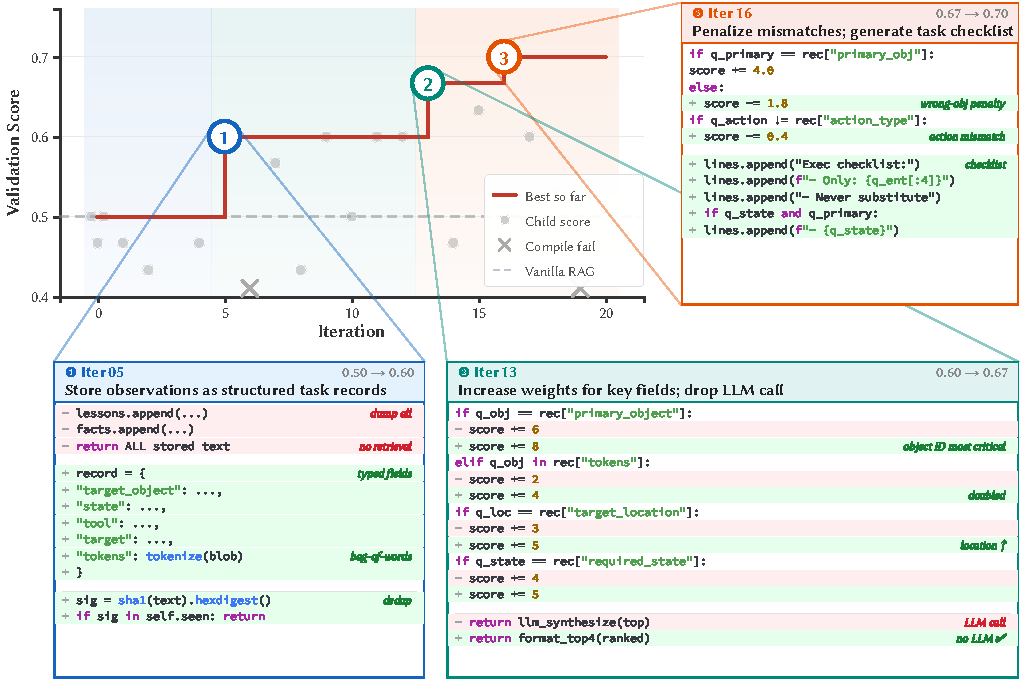
\includegraphics[width=\textwidth]{figures/trajectory/fig3_d3.pdf}
\caption{\textbf{ALFWorld evolution trajectory.}
The main panel plots each child program's validation score and the best score so far across 20 evolution iterations, with crosses marking compile failures and the dashed line marking the Vanilla RAG baseline.
Numbered panels highlight representative code changes that structure task records, reweight retrieval, and add mismatch penalties and execution checklists for selecting the next action.}
\label{fig:evolution-trajectory}
\vspace{-1em}
\end{figure*}



\section{Results}
\label{sec:results}

We organize the analysis around three questions: whether memory-program search improves task performance, whether the resulting programs differ structurally across tasks, and which evolved components drive the gains.

\paragraph{Reflective code evolution progressively discovers better memory programs.}\looseness=-1
Table~\ref{tab:main-results} shows that \sysname{} achieves the highest score on seven of eight reported metrics.
Compared with the best baseline in each winning metric, the relative improvement is up to 31\%, with the largest gains on LoCoMo and PRBench.
The strongest baseline varies by task, indicating that existing memory methods have task-dependent strengths.
GEPA is competitive on ALFWorld and PRBench, while Mem0, GEPA+Vector Search, and Dynamic Cheatsheet lead the baselines on LoCoMo and HealthBench.
In comparison, \sysname{} achieves the best overall performance.
This pattern suggests that executable code search reaches useful memory designs beyond the strongest fixed baselines.
Figure~\ref{fig:evolution-trajectory} shows the ALFWorld evolution trajectory.
The evolved memory program improves steadily over iterations, with the reflector producing task-specific changes at different stages of search.
Early edits build a usable task-record schema that captures objects, locations, and state changes from demonstrations.
Later edits refine retrieval weights and add action-selection checks, allowing the agent to retrieve more relevant trajectory patterns and choose actions more reliably.

\paragraph{Different tasks produce structurally distinct optimal memory programs.}
% Table 2: Ablation study on LoCoMo
\begin{wraptable}{r}{0.44\textwidth}
    % \vspace{-1.2em}
    \centering
    \footnotesize
    \caption{\textbf{Ablation study on LoCoMo.}
    Rows report the full system and variants that remove or alter one design choice; metric is token F1.
    $\Delta$ reports absolute change from the full system.}
    % \vspace{-0.5em}
    \label{tab:ablation}
    \begin{tabular}{@{}lcc@{}}
        \toprule
        \rowcolor{gray!10}
        \textbf{Variant} & \textbf{F1} & \textbf{$\Delta$} \\
        \midrule
        \rowcolor{green!10}
        \sysname{}                           & 0.459  & ---      \\
        \quad $-$ Instruction                 & 0.353  & $-$0.106 \\
        \quad $-$ Code                        & 0.256  & $-$0.203 \\
        \quad Max parent selection          & 0.381  & $-$0.078 \\
        \quad $-$ Diversity                   & 0.318  & $-$0.141 \\
        \bottomrule
    \end{tabular}%
    \vspace{-1em}
\end{wraptable}


% fig5.tex — Program embedding landscape (Observation 4)
% Generated from fig5.html via Puppeteer → fig5.pdf

\begin{figure*}[t]
\centering
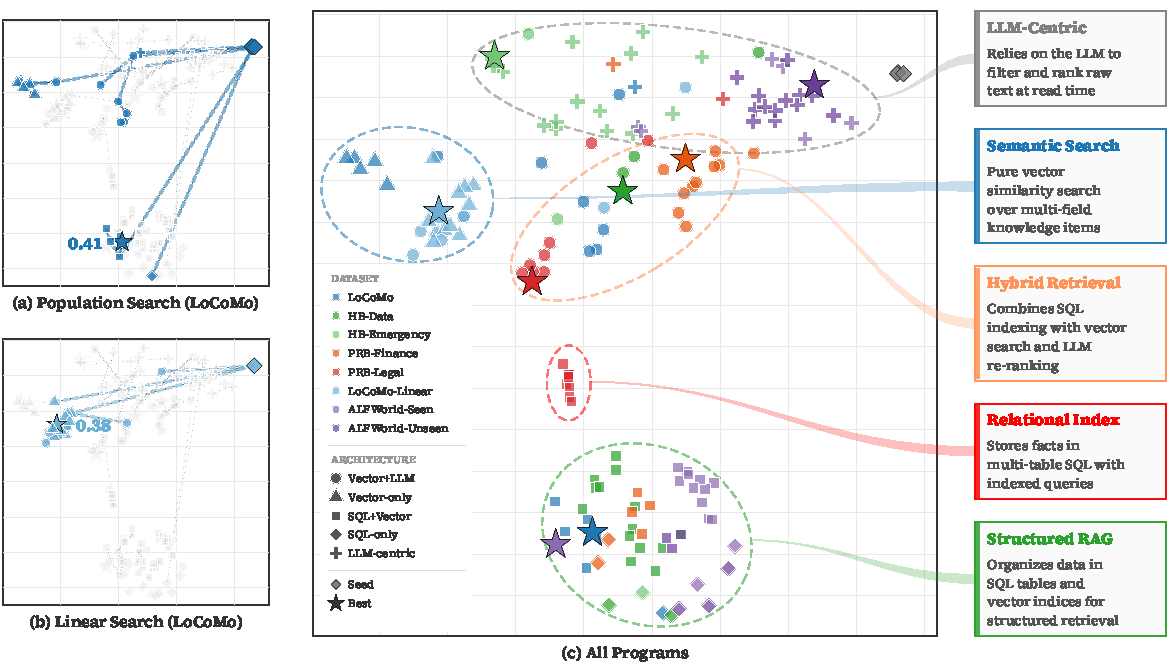
\includegraphics[width=\textwidth]{figures/landscape/fig5.pdf}
\caption{%
  \textbf{Program embedding landscape.}
  Each evolved program is embedded with a code embedding model and projected to 2D via t-SNE~\citep{vandermaaten2008tsne}.
  \textbf{(a,\,b)}~Population-based search (\sysname{}) and linear search, with colored edges tracing parent-child lineage.
  \textbf{(c)}~All programs from the evaluated configurations and the LoCoMo linear-search ablation, colored by configuration.
  Marker shapes denote the storage architecture discovered by evolution: circles for vector\,+\,LLM, triangles for vector-only, squares for SQL\,+\,vector, rotated squares for SQL-only, and crosses for LLM-centric designs; diamonds mark seed programs and stars mark the best program for each configuration.
}
\label{fig:landscape}
\end{figure*}


To understand how \sysname{} adapts memory program structure to different tasks, we visualize the program embedding landscape accumulated during evolution (Figure~\ref{fig:landscape}).
For each task and iteration, we first sanitize the program by replacing strings and variable names with placeholders so that the embedding emphasizes structural differences.
We then embed the sanitized programs with a code embedding model and project them with t-SNE~\citep{vandermaaten2008tsne}.
The projection places the best programs for different benchmark configurations in separate regions, with markers indicating different storage architectures.
For example, the best ALFWorld program uses a compact SQLite action cache with read-time LLM synthesis.
The best LoCoMo program uses ChromaDB semantic retrieval together with SQLite lexical and metadata scoring.
Appendix~\ref{app:evolved-comparison} reports structural summaries, and the supplementary material includes full code for all best programs.

% Fig 4: Cross-task transfer of evolved memory programs
\begin{figure*}[t]
\centering
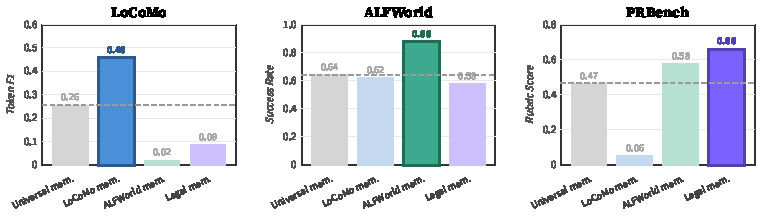
\includegraphics[width=\textwidth]{figures/comparison/fig4.pdf}
\caption{\textbf{Cross-task transfer of evolved memory programs.}
Each panel fixes one target benchmark and compares memory programs evolved on different source benchmarks.
Highlighted bars mark native-task programs, and the dashed line marks the universal seed baseline.}
\label{fig:task-optimized-memory}
\vspace{-1em}
\end{figure*}


To further test whether these structures are task-specific, we evaluate the best evolved program from each source task on other target tasks (Figure~\ref{fig:task-optimized-memory}).
In all three targets, the native evolved program outperforms transferred programs from other benchmarks.
Five of six transferred programs perform worse than the universal seed baseline.
This pattern suggests that memory program structure should be optimized together with the target task.


\paragraph{Joint evolution of structure and policy enables task-specific adaptation.}
Table~\ref{tab:ablation} isolates key design choices on LoCoMo.
Each variant removes one component of \sysname{}: \textit{$-$\,Instruction} lets only the code evolve and keeps the prompt instructions fixed; \textit{$-$\,Code} does the opposite, evolving only the prompt instructions while keeping the code at the Vector Search seed; \textit{Max parent selection} always picks the highest-scoring parent instead of sampling by softmax; and \textit{$-$\,Diversity} drops the population pool and mutates only the current best program at each iteration.
\textit{$-$\,Code} gives the largest drop, reducing F1 by 0.203.
\textit{$-$\,Instruction} reduces F1 by 0.106.
The full system also scores above \textit{Max parent selection} and \textit{$-$\,Diversity}.
These results indicate that joint optimization of program Logic and Instruction gives the strongest LoCoMo result.

% === Table 2: Ablation ===
